\documentclass[8pt,apectratio=169]{beamer}

\usetheme[progressbar=frametitle]{metropolis}
\usepackage{appendixnumberbeamer}
\usepackage[style=authoryear, backend=bibtex8, natbib=true, maxcitenames=2]{biblatex}

\usepackage[utf8]{inputenc} % utf8x  defines more symbols, but may cause compatible problems
\usepackage{lmodern,textcomp} % Latin Modern fonts, contains €

\usepackage{graphicx}
\usepackage{import}

\usepackage{booktabs}
\usepackage[scale=2]{ccicons}

\usepackage{pgfplots}
\usepgfplotslibrary{dateplot}

\usepackage{xspace}
\newcommand{\themename}{\textbf{\textsc{metropolis}}\xspace}

% Math
\usepackage{amsmath}
\usepackage{bm} % bold symbol in math mode

% Optional packages
\usepackage{xcolor}
\usepackage{multicol}
\usepackage{hyperref}
\usepackage[super,negative]{nth} % allows writing 1st, 2nd, 3rd with superscript
\usepackage{ulem} % use the "sout" tag to "strikethrough" text
\usepackage{tcolorbox}

% Select what to do with command \comment:
  % \newcommand{\comment}[1]{}  %comments not shown
  % \newcommand{\comment}[1]{\par {\bfseries \color{blue} #1 \par}} %comments shown
% Select what to do with todonotes: i.e. \todo{}, \todo[inline]{}
  % \usepackage[disable]{todonotes} % notes not shown
  % \usepackage[draft]{todonotes}   % notes shown

%\numberwithin{equation}{section}

%\addbibresource{references}

\titlegraphic{\hfill 
\includegraphics[width=0.15 \textwidth]{figures/logo}}
\title{Microeconomics III, Ex. Class 4: Problem Set 1\footnote{Slides created for exercise class 4, with reservation for possible errors.\\}}
\author{Thor Donsby Noe (\href{mailto:thor.noe@econ.ku.dk}{thor.noe@econ.ku.dk})}
\date{September 11 2019} % \today
\institute{\normalsize Department of Economics, University of Copenhagen}

    % \definecolor{BlueTOL}{HTML}{222255}
    \definecolor{BrownTOL}{HTML}{666633}
    \definecolor{GreenTOL}{HTML}{225522}
    % \setbeamercolor{normal text}{fg=BlueTOL,bg=white}
    \setbeamercolor{alerted text}{fg=BrownTOL}
    \setbeamercolor{example text}{fg=GreenTOL}
    \setbeamercolor{background canvas}{bg=white}

    \setbeamercolor{block title alerted}{use=alerted text,
        fg=alerted text.fg,
        bg=alerted text.bg!80!alerted text.fg}
    \setbeamercolor{block body alerted}{use={block title alerted, alerted text},
        fg=alerted text.fg,
        bg=block title alerted.bg!50!alerted text.bg}
    \setbeamercolor{block title example}{use=example text,
        fg=example text.fg,
        bg=example text.bg!80!example text.fg}
    \setbeamercolor{block body example}{use={block title example, example text},
        fg=example text.fg,
        bg=block title example.bg!50!example text.bg}

\begin{document}

\begin{frame}{PS4, Ex. 1.b (A): MSNE and best-response functions}
  \begin{multicols}{2}
    \begin{itemize}
      \item[(b)] Find all equilibria (pure and mixed), first analytically and then through plotting the BR functions.
    \end{itemize}
    \begin{table}
      \begin{tabular}{cl|c|c|}
          & \multicolumn{1}{c}{} & \multicolumn{2}{c}{Player 2}\\
          \parbox[t]{1mm}{\multirow{3}{*}{\rotatebox[origin=r]{90}{Player 1}}}
          & \multicolumn{1}{c}{} & \multicolumn{1}{c}{L (q)} & \multicolumn{1}{c}{R (1-q)} \\\cline{3-4}
          & T (p) & 1, 1 & 0, 0 \\\cline{3-4}
          & B (1-p) & 1, 0 & 2, 1 \\\cline{3-4}
      \end{tabular}
    \end{table}
    \textbf{\textit{Highlight the best responses in pure strategies.}}
  \vfill\null \columnbreak
  \vfill\null
  \end{multicols}
\end{frame}
\begin{frame}{PS4, Ex. 1.b (A): MSNE and best-response functions}
  \begin{multicols}{2}
    \begin{itemize}
      \item[(b)] Find all equilibria (pure and mixed), first analytically and then through plotting the BR functions.
    \end{itemize}
    \begin{table}
      \begin{tabular}{cl|c|c|}
        & \multicolumn{1}{c}{} & \multicolumn{2}{c}{\color{blue}Player 2}\\
        \parbox[t]{1mm}{\multirow{3}{*}{\rotatebox[origin=r]{90}{\color{red}Player 1}}}
        & \multicolumn{1}{c}{} & \multicolumn{1}{c}{L (q)} & \multicolumn{1}{c}{R (1-q)} \\\cline{3-4}
        & T (p) & \textcolor{red}{1}, \textcolor{blue}{1} & 0, 0 \\\cline{3-4}
        & B (1-p) & \textcolor{red}{1}, 0 & \textcolor{red}{2}, \textcolor{blue}{1} \\\cline{3-4}
      \end{tabular}
    \end{table}
    \textbf{\textit{For which values of q is Player 1 indifferent?}}\\\medskip
    Find $q$ such that Player 1 expects to have equal payoffs from playing $T$ and $B$:
    \begin{align*}
      E[u_1(T)|q]&=E[u_1(B)|q]\\
       &=
    \end{align*}
  \vfill\null \columnbreak
  \vfill\null
  \end{multicols}
\end{frame}
\begin{frame}{PS4, Ex. 1.b (A): MSNE and best-response functions}
  \begin{multicols}{2}
    \begin{itemize}
      \item[(b)] Find all equilibria (pure and mixed), first analytically and then through plotting the BR functions.
    \end{itemize}
    \begin{table}
      \begin{tabular}{cl|c|c|}
        & \multicolumn{1}{c}{} & \multicolumn{2}{c}{\color{blue}Player 2}\\
        \parbox[t]{1mm}{\multirow{3}{*}{\rotatebox[origin=r]{90}{\color{red}Player 1}}}
        & \multicolumn{1}{c}{} & \multicolumn{1}{c}{L (q)} & \multicolumn{1}{c}{R (1-q)} \\\cline{3-4}
        & T (p) & \textcolor{red}{1}, \textcolor{blue}{1} & 0, 0 \\\cline{3-4}
        & B (1-p) & \textcolor{red}{1}, 0 & \textcolor{red}{2}, \textcolor{blue}{1} \\\cline{3-4}
      \end{tabular}
    \end{table}
    Find $q$ such that Player 1 expects to have equal payoffs from playing $T$ and $B$:
    \begin{align*}
      E[u_1(T)|q]&=E[u_1(B)|q]\\
      q &= q + 2(1-q) \Leftrightarrow q = 1
    \end{align*}
    \textbf{\textit{For which values of p is Player 2 indifferent?}}\\\medskip
    Find $p$ such that Player 2 expect to have equal payoffs from playing $L$ and $R$:
    \begin{align*}
      E[u_2(L)|p]&=E[u_2(R)|p]\\
       &=
    \end{align*}
  \vfill\null \columnbreak
  \vfill\null
  \end{multicols}
\end{frame}
\begin{frame}{PS4, Ex. 1.b (A): MSNE and best-response functions}
  \begin{multicols}{2}
    \begin{itemize}
      \item[(b)] Find all equilibria (pure and mixed), first analytically and then through plotting the BR functions.
    \end{itemize}
    \begin{table}
      \begin{tabular}{cl|c|c|}
        & \multicolumn{1}{c}{} & \multicolumn{2}{c}{\color{blue}Player 2}\\
        \parbox[t]{1mm}{\multirow{3}{*}{\rotatebox[origin=r]{90}{\color{red}Player 1}}}
        & \multicolumn{1}{c}{} & \multicolumn{1}{c}{L (q)} & \multicolumn{1}{c}{R (1-q)} \\\cline{3-4}
        & T (p) & \textcolor{red}{1}, \textcolor{blue}{1} & 0, 0 \\\cline{3-4}
        & B (1-p) & \textcolor{red}{1}, 0 & \textcolor{red}{2}, \textcolor{blue}{1} \\\cline{3-4}
      \end{tabular}
    \end{table}
    Find $q$ such that Player 1 expects to have equal payoffs from playing $T$ and $B$:
    \begin{align*}
      E[u_1(T)|q]&=E[u_1(B)|q]\\
      q &= q + 2(1-q) \Leftrightarrow q = 1
    \end{align*}
    Find $p$ such that Player 2 expect to have equal payoffs from playing $L$ and $R$:
    \begin{align*}
      E[u_2(L)|p]&=E[u_2(R)|p]\\
      p &= 1-p \Leftrightarrow p = \frac{1}{2}
    \end{align*}
    and chooses $q=1$ for $p>1/2$.\\\medskip
    \textbf{\textit{Write up all NE (pure and mixed).}}
  \vfill\null \columnbreak
  \vfill\null
  \end{multicols}
\end{frame}
\begin{frame}{PS4, Ex. 1.b (A): MSNE and best-response functions}
  \begin{multicols}{2}
    \begin{itemize}
      \item[(b)] Find all NE, first analytically:
    \end{itemize}
    \begin{table}
      \begin{tabular}{cl|c|c|}
        & \multicolumn{1}{c}{} & \multicolumn{2}{c}{\color{blue}Player 2}\\
        \parbox[t]{1mm}{\multirow{3}{*}{\rotatebox[origin=r]{90}{\color{red}Player 1}}}
        & \multicolumn{1}{c}{} & \multicolumn{1}{c}{L (q)} & \multicolumn{1}{c}{R (1-q)} \\\cline{3-4}
        & T (p) & \textcolor{red}{1}, \textcolor{blue}{1} & 0, 0 \\\cline{3-4}
        & B (1-p) & \textcolor{red}{1}, 0 & \textcolor{red}{2}, \textcolor{blue}{1} \\\cline{3-4}
      \end{tabular}
    \end{table}
    Player 1 is indifferent for:
    \begin{align*}
      E[u_1(T)|q]&=E[u_1(B)|q]\\
      q &= q + 2(1-q) \Leftrightarrow q = 1
    \end{align*}
    Player 2 is indifferent for:
    \begin{align*}
      E[u_2(L)|p]&=E[u_2(R)|p]\\
      p &= 1-p \Leftrightarrow p = \frac{1}{2}
    \end{align*}
    and chooses $q=1$ for $p>1/2$.\\\medskip
    The pure and mixed NE, $(p^{*},q^{*})$, are:
    \begin{align*}
      \left\{(0,0);(1,1);\left(p\in\left[\frac{1}{2},1\right),q=1\right)\right\}
    \end{align*}
  \vfill\null \columnbreak
  \vfill\null
  \end{multicols}
\end{frame}
\begin{frame}{PS4, Ex. 1.b (A): MSNE and best-response functions}
  \begin{multicols}{2}
    \begin{itemize}
      \item[(b)] Find all NE, first analytically:
    \end{itemize}
    \begin{table}
      \begin{tabular}{cl|c|c|}
        & \multicolumn{1}{c}{} & \multicolumn{2}{c}{\color{blue}Player 2}\\
        \parbox[t]{1mm}{\multirow{3}{*}{\rotatebox[origin=r]{90}{\color{red}Player 1}}}
        & \multicolumn{1}{c}{} & \multicolumn{1}{c}{L (q)} & \multicolumn{1}{c}{R (1-q)} \\\cline{3-4}
        & T (p) & \textcolor{red}{1}, \textcolor{blue}{1} & 0, 0 \\\cline{3-4}
        & B (1-p) & \textcolor{red}{1}, 0 & \textcolor{red}{2}, \textcolor{blue}{1} \\\cline{3-4}
      \end{tabular}
    \end{table}
    Player 1 is indifferent for:
    \begin{align*}
      E[u_1(T)|q]&=E[u_1(B)|q]\\
      q &= q + 2(1-q) \Leftrightarrow q = 1
    \end{align*}
    Player 2 is indifferent for:
    \begin{align*}
      E[u_2(L)|p]&=E[u_2(R)|p]\\
      p &= 1-p \Leftrightarrow p = \frac{1}{2}
    \end{align*}
    and chooses $q=1$ for $p>1/2$.\\\medskip
    The pure and mixed NE, $(p^{*},q^{*})$, are:
    \begin{align*}
      \left\{(0,0);(1,1);\left(p\in\left[\frac{1}{2},1\right),q=1\right)\right\}
    \end{align*}
    \textbf{\textit{Write up Player 1's best-response (BR) function, $\bm{p^{*}(q)}$}}
  \vfill\null \columnbreak
    \begin{align*}
      BR_1(q)=\left\{ \right.
    \end{align*}
  \vfill\null
  \end{multicols}
\end{frame}
\begin{frame}{PS4, Ex. 1.b (A): MSNE and best-response functions}
  \begin{multicols}{2}
    \begin{itemize}
      \item[(b)] Find all NE, first analytically:
    \end{itemize}
    \begin{table}
      \begin{tabular}{cl|c|c|}
        & \multicolumn{1}{c}{} & \multicolumn{2}{c}{\color{blue}Player 2}\\
        \parbox[t]{1mm}{\multirow{3}{*}{\rotatebox[origin=r]{90}{\color{red}Player 1}}}
        & \multicolumn{1}{c}{} & \multicolumn{1}{c}{L (q)} & \multicolumn{1}{c}{R (1-q)} \\\cline{3-4}
        & T (p) & \textcolor{red}{1}, \textcolor{blue}{1} & 0, 0 \\\cline{3-4}
        & B (1-p) & \textcolor{red}{1}, 0 & \textcolor{red}{2}, \textcolor{blue}{1} \\\cline{3-4}
      \end{tabular}
    \end{table}
    Player 1 is indifferent for:
    \begin{align*}
      E[u_1(T)|q]&=E[u_1(B)|q]\\
      q &= q + 2(1-q) \Leftrightarrow q = 1
    \end{align*}
    Player 2 is indifferent for:
    \begin{align*}
      E[u_2(L)|p]&=E[u_2(R)|p]\\
      p &= 1-p \Leftrightarrow p = \frac{1}{2}
    \end{align*}
    and chooses $q=1$ for $p>1/2$.\\\medskip
    The pure and mixed NE, $(p^{*},q^{*})$, are:
    \begin{align*}
      \left\{(0,0);(1,1);\left(p\in\left[\frac{1}{2},1\right),q=1\right)\right\}
    \end{align*}
    \textbf{\textit{Plot Player 1's best-response (BR) function, $\bm{p^{*}(q)}$}}
  \vfill\null \columnbreak
    Then through plotting the BR functions:
    \vspace{-8pt}
    \begin{align*}
      BR_1(q)=\left\{ \begin{array}{lcl}
          p=0       & \text{if} & q<1 \\
          p\in[0,1] & \text{if} & q=1
      \end{array}\right.
    \end{align*}
    \vspace{-8pt}
    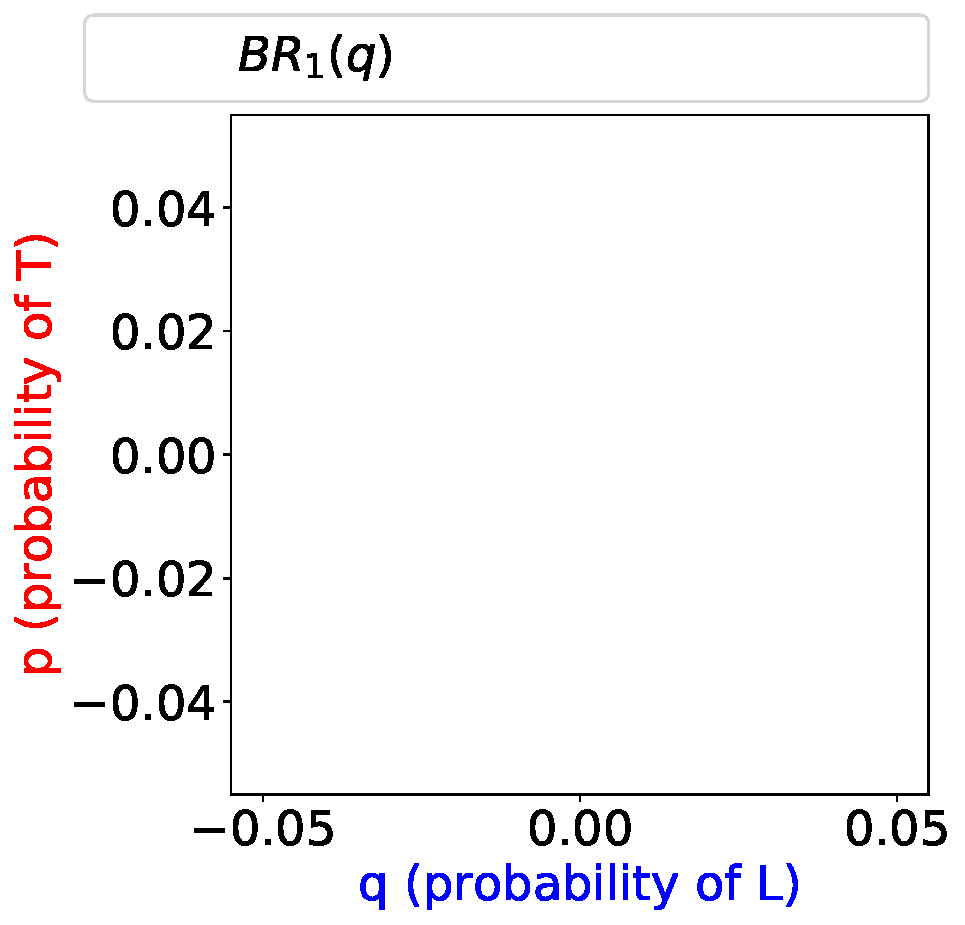
\includegraphics[width=\columnwidth]{figures/empty_plot_}
  \vfill\null
  \end{multicols}
\end{frame}
\begin{frame}{PS4, Ex. 1.b (A): MSNE and best-response functions}
  \begin{multicols}{2}
    \begin{itemize}
      \item[(b)] Find all NE, first analytically:
    \end{itemize}
    \begin{table}
      \begin{tabular}{cl|c|c|}
        & \multicolumn{1}{c}{} & \multicolumn{2}{c}{\color{blue}Player 2}\\
        \parbox[t]{1mm}{\multirow{3}{*}{\rotatebox[origin=r]{90}{\color{red}Player 1}}}
        & \multicolumn{1}{c}{} & \multicolumn{1}{c}{L (q)} & \multicolumn{1}{c}{R (1-q)} \\\cline{3-4}
        & T (p) & \textcolor{red}{1}, \textcolor{blue}{1} & 0, 0 \\\cline{3-4}
        & B (1-p) & \textcolor{red}{1}, 0 & \textcolor{red}{2}, \textcolor{blue}{1} \\\cline{3-4}
      \end{tabular}
    \end{table}
    Player 1 is indifferent for:
    \begin{align*}
      E[u_1(T)|q]&=E[u_1(B)|q]\\
      q &= q + 2(1-q) \Leftrightarrow q = 1
    \end{align*}
    Player 2 is indifferent for:
    \begin{align*}
      E[u_2(L)|p]&=E[u_2(R)|p]\\
      p &= 1-p \Leftrightarrow p = \frac{1}{2}
    \end{align*}
    and chooses $q=1$ for $p>1/2$.\\\medskip
    The pure and mixed NE, $(p^{*},q^{*})$, are:
    \begin{align*}
      \left\{(0,0);(1,1);\left(p\in\left[\frac{1}{2},1\right),q=1\right)\right\}
    \end{align*}
    \textbf{\textit{Write up Player 2's BR function, $\bm{q^{*}(p)}$}}
  \vfill\null \columnbreak
    Then through plotting the BR functions:
    \vspace{-8pt}
    \begin{align*}
      BR_1(q)&=\left\{ \begin{array}{lcl}
          p=0       & \text{if} & q<1 \\
          p\in[0,1] & \text{if} & q=1
      \end{array}\right.\\
      BR_2(p)&=
    \end{align*}
    \vspace{-8pt}
    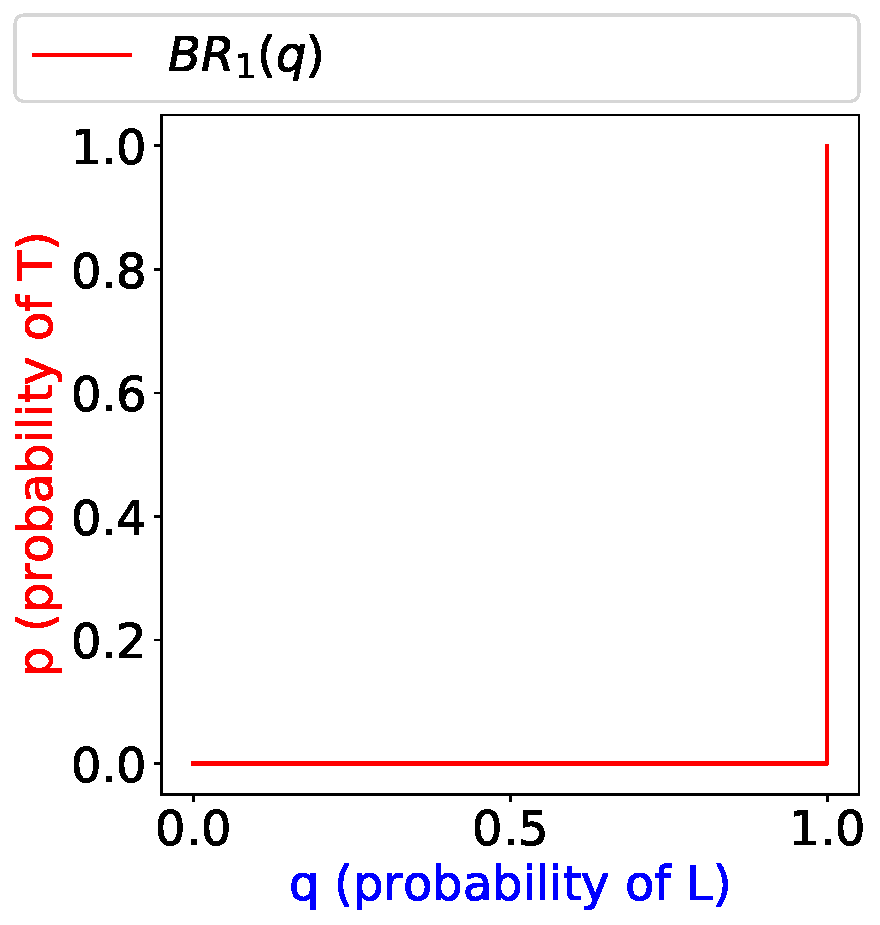
\includegraphics[width=\columnwidth]{figures/1b_}
  \vfill\null
  \end{multicols}
\end{frame}
\begin{frame}{PS4, Ex. 1.b (A): MSNE and best-response functions}
  \begin{multicols}{2}
    \begin{itemize}
      \item[(b)] Find all NE, first analytically:
    \end{itemize}
    \begin{table}
      \begin{tabular}{cl|c|c|}
        & \multicolumn{1}{c}{} & \multicolumn{2}{c}{\color{blue}Player 2}\\
        \parbox[t]{1mm}{\multirow{3}{*}{\rotatebox[origin=r]{90}{\color{red}Player 1}}}
        & \multicolumn{1}{c}{} & \multicolumn{1}{c}{L (q)} & \multicolumn{1}{c}{R (1-q)} \\\cline{3-4}
        & T (p) & \textcolor{red}{1}, \textcolor{blue}{1} & 0, 0 \\\cline{3-4}
        & B (1-p) & \textcolor{red}{1}, 0 & \textcolor{red}{2}, \textcolor{blue}{1} \\\cline{3-4}
      \end{tabular}
    \end{table}
    Player 1 is indifferent for:
    \begin{align*}
      E[u_1(T)|q]&=E[u_1(B)|q]\\
      q &= q + 2(1-q) \Leftrightarrow q = 1
    \end{align*}
    Player 2 is indifferent for:
    \begin{align*}
      E[u_2(L)|p]&=E[u_2(R)|p]\\
      p &= 1-p \Leftrightarrow p = \frac{1}{2}
    \end{align*}
    and chooses $q=1$ for $p>1/2$.\\\medskip
    The pure and mixed NE, $(p^{*},q^{*})$, are:
    \begin{align*}
      \left\{(0,0);(1,1);\left(p\in\left[\frac{1}{2},1\right),q=1\right)\right\}
    \end{align*}
    \textbf{\textit{Plot Player 2's BR function, $\bm{q^{*}(p)}$}}
  \vfill\null \columnbreak
    Then through plotting the BR functions:
    \vspace{-8pt}
    \begin{align*}
      BR_1(q)&=\left\{ \begin{array}{lcl}
          p=0       & \text{if} & q<1 \\
          p\in[0,1] & \text{if} & q=1
      \end{array}\right. \\
      BR_2(p)&=\left\{ \begin{array}{lcl}
          q=0       & \text{if} & p<1/2  \\
          q\in[0,1] & \text{if} & p=1/2 \\
          q=1       & \text{if} & p>1/2
      \end{array}\right.
    \end{align*}
    \vspace{-8pt}
    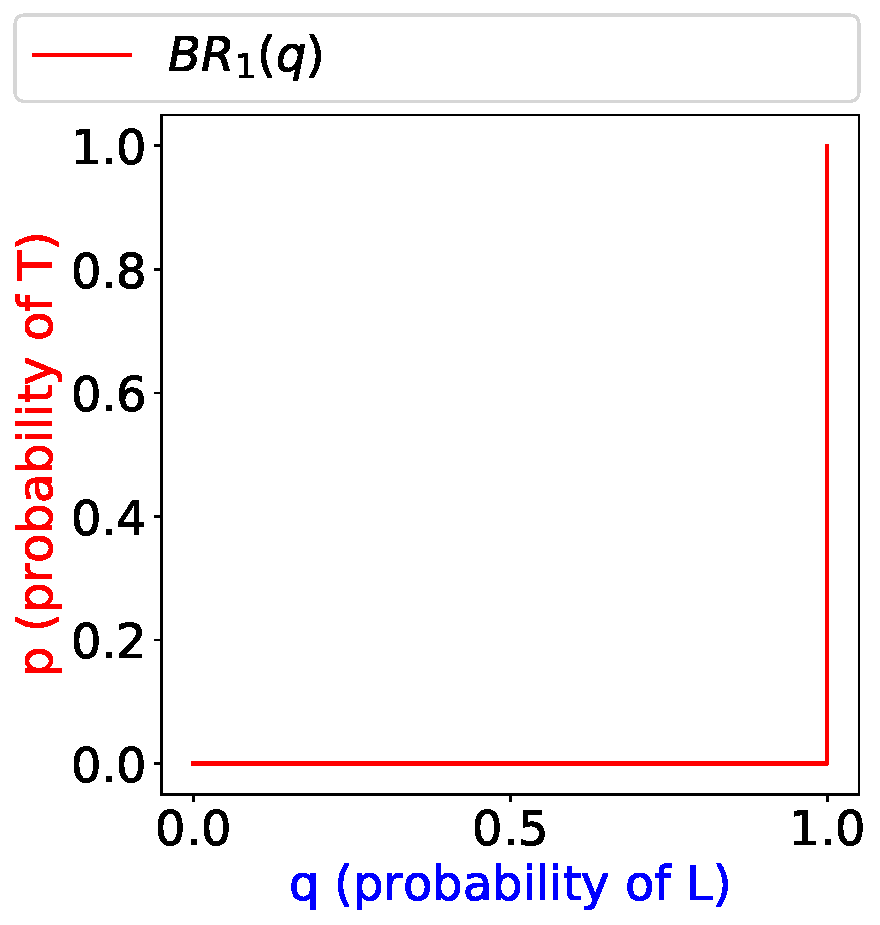
\includegraphics[width=\columnwidth]{figures/1b_}
  \vfill\null
  \end{multicols}
\end{frame}
\begin{frame}{PS4, Ex. 1.b (A): MSNE and best-response functions}
  \begin{multicols}{2}
    \begin{itemize}
      \item[(b)] Find all NE, first analytically:
    \end{itemize}
    \begin{table}
      \begin{tabular}{cl|c|c|}
        & \multicolumn{1}{c}{} & \multicolumn{2}{c}{\color{blue}Player 2}\\
        \parbox[t]{1mm}{\multirow{3}{*}{\rotatebox[origin=r]{90}{\color{red}Player 1}}}
        & \multicolumn{1}{c}{} & \multicolumn{1}{c}{L (q)} & \multicolumn{1}{c}{R (1-q)} \\\cline{3-4}
        & T (p) & \textcolor{red}{1}, \textcolor{blue}{1} & 0, 0 \\\cline{3-4}
        & B (1-p) & \textcolor{red}{1}, 0 & \textcolor{red}{2}, \textcolor{blue}{1} \\\cline{3-4}
      \end{tabular}
    \end{table}
    Player 1 is indifferent for:
    \begin{align*}
      E[u_1(T)|q]&=E[u_1(B)|q]\\
      q &= q + 2(1-q) \Leftrightarrow q = 1
    \end{align*}
    Player 2 is indifferent for:
    \begin{align*}
      E[u_2(L)|p]&=E[u_2(R)|p]\\
      p &= 1-p \Leftrightarrow p = \frac{1}{2}
    \end{align*}
    and chooses $q=1$ for $p>1/2$.\\\medskip
    The pure and mixed NE, $(p^{*},q^{*})$, are:
    \begin{align*}
      \left\{(0,0);(1,1);\left(p\in\left[\frac{1}{2},1\right),q=1\right)\right\}
    \end{align*}
  \vfill\null \columnbreak
    Then through plotting the BR functions:
    \vspace{-8pt}
    \begin{align*}
      BR_1(q)&=\left\{ \begin{array}{lcl}
          p=0       & \text{if} & q<1 \\
          p\in[0,1] & \text{if} & q=1
      \end{array}\right. \\
      BR_2(p)&=\left\{ \begin{array}{lcl}
          q=0       & \text{if} & p<1/2  \\
          q\in[0,1] & \text{if} & p=1/2 \\
          q=1       & \text{if} & p>1/2
      \end{array}\right.
    \end{align*}
    \vspace{-8pt}
    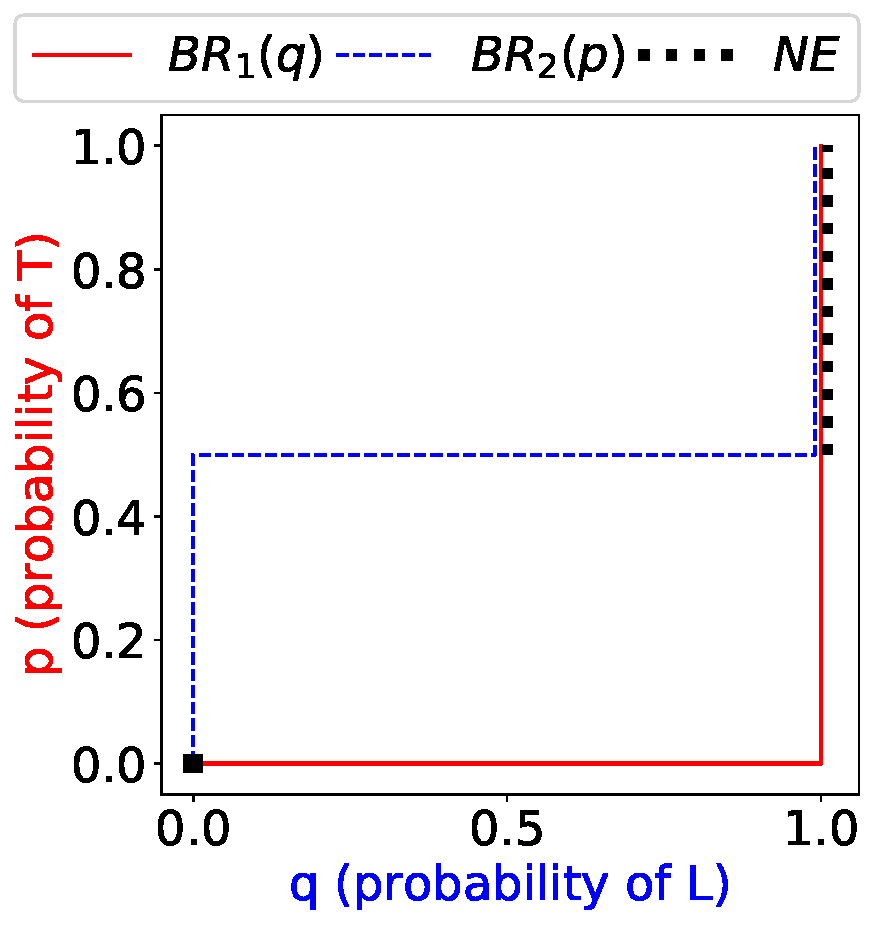
\includegraphics[width=\columnwidth]{figures/1b}
  \vfill\null
  \end{multicols}
\end{frame}

\end{document}
